DARWIN is a high-level description of an algorithm that can be used to solve
a~multi-objective optimization problem. It is a~list of steps to execute and
calculations to perform. Therefore, one does not need a computer to realize
the decision-making process. However, in practice it is almost impossible to
complete all the steps without a dedicated software application. Moreover, to
evaluate the method's performance one needs to repeat the experiments several
times.

For the reasons stated above it was required to implement the method as a
computer program. This chapter describes technologies used for the DARWIN's
implementation and an experiment framework development.

\section{The method's implementation}

\subsection{The environment}

The environment in which DARWIN has to function is not empty; thus it has to
be taken into account during the development of the implementation. It is
shown in~fig.~\ref{environ}. DARWIN is a~realization of an interactive
process, therefore a way of communication with the decision maker is
required. Another restriction is imposed by the need of inducing decision
rules from the DM's evaluated examples of solutions.

\begin{figure}
  \centering 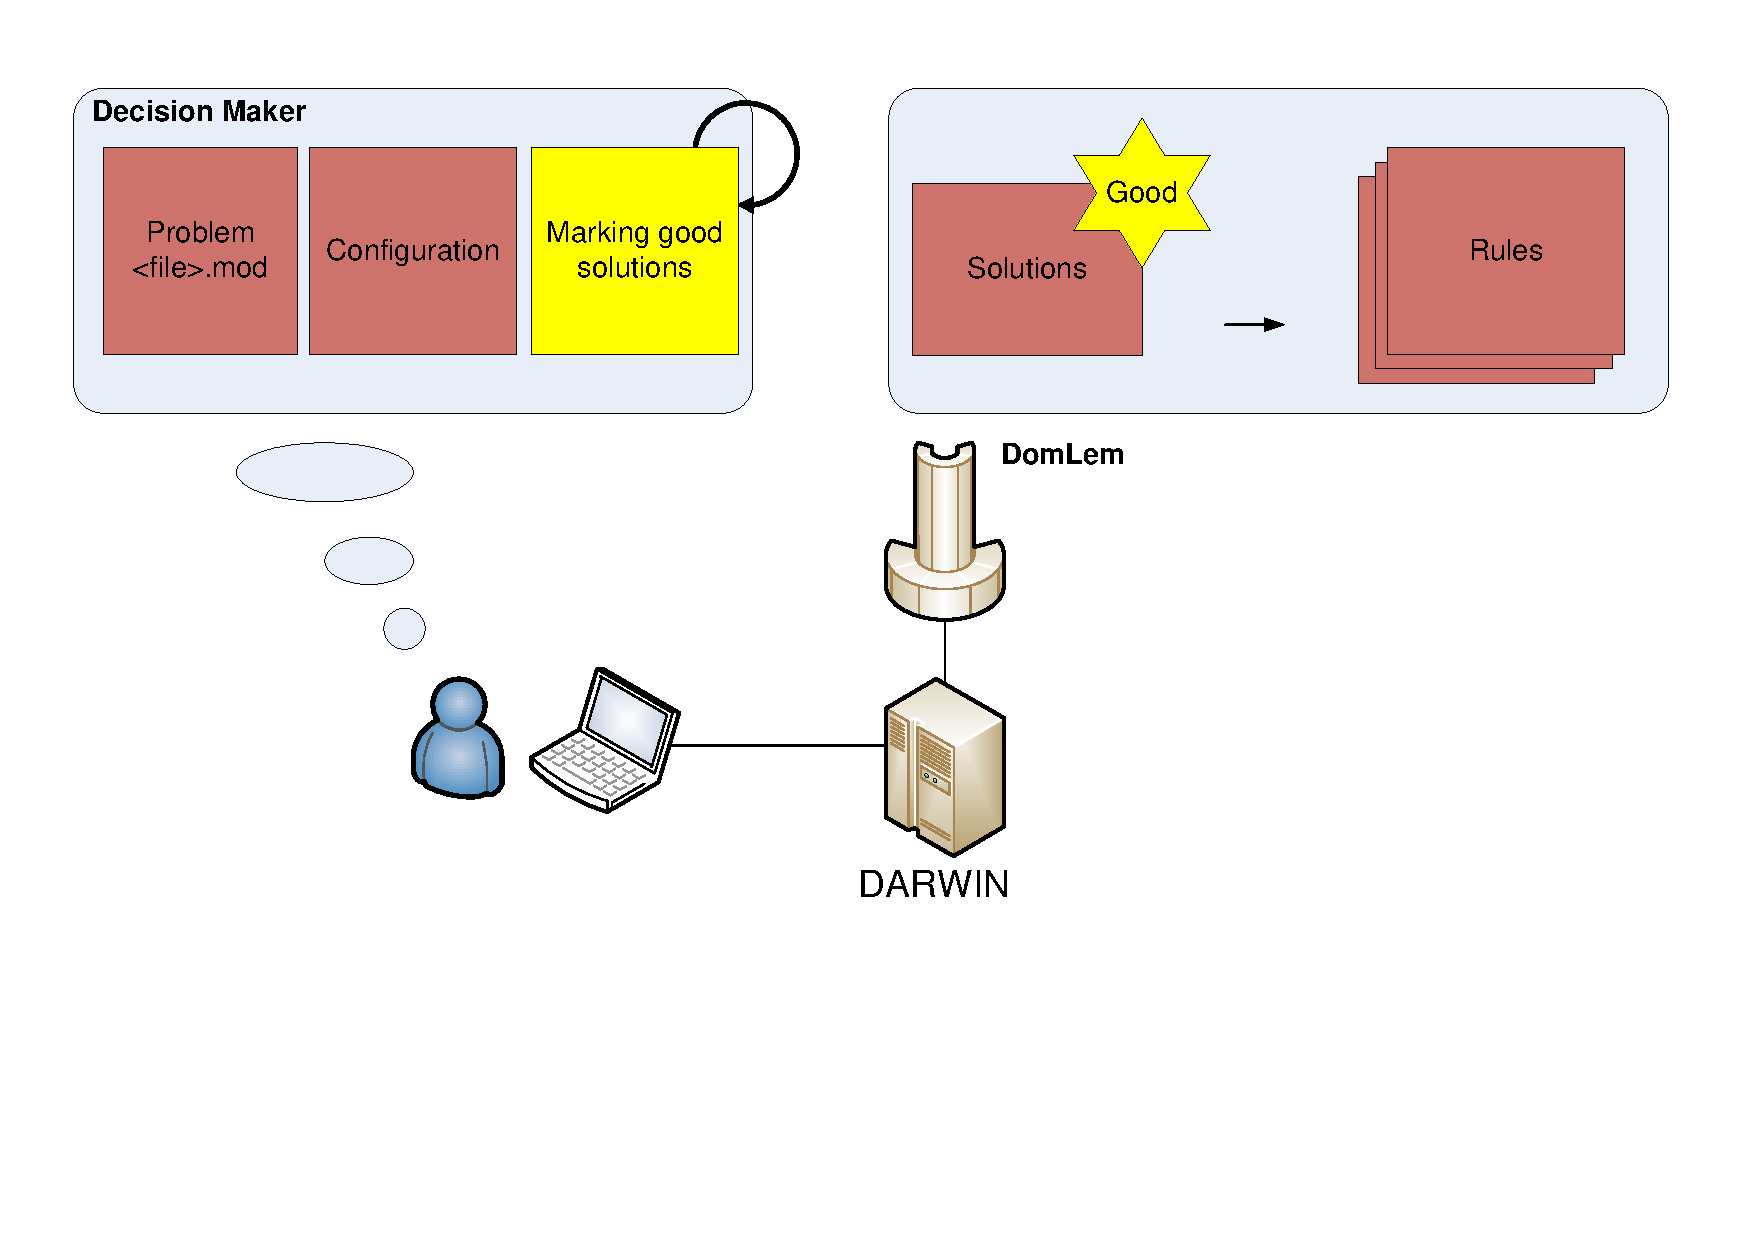
\includegraphics[scale=0.5]{img/environ}
  \caption{DARWIN's environment}
  \label{environ}
\end{figure}

The decision maker has to provide a problem he or she wants to solve. It can
be done in a model file. If one wants to change the default parameters'
values, then a~configuration file with the values is also required. Moreover,
during the algorithm's run, presence of the decision maker is needed in order
to select ``good'' solutions from the provided ones. Consult the user manual
([inref]) for more details on the file formats. The parameters are described
later in this section.

Decision rules store the DM's preferences, therefore they are a~symbolic
representation of trade-offs he or she is willing to make, as well as the
importance of each criterion. They ensure robustness of the resulting
solutions because of an underlying DRSA framework. The rules are a~very
important part of the method. Thus, a~way --- an algorithm --- to generate
them is needed. In the method's description provided in [ref], a~phase of
obtaining the rules is treated as a~black box. It is assumed that a~component
able to generate rules from the DM's selection exists. Details are omitted ---
it is up to an analyst (or to a~developer of an implementation) to use
a~software component he or she finds feasible.

The implementation of the DRSA framework, being able to induce decision rules
from a~given set of examples is a complex task, both in terms of possible
technical challenges as well as conceptual and scientific work that needs to
be carried out. Such a software application deserves a paper of its
own. Therefore, the author decided to use an existing implementation in order
to focus on the DARWIN method. Java Rough Set (jRS) --- a~project of the
Laboratory of Intelligent Decision Support Systems at Poznań University of
Technology that aims at providing DRSA framework implementation in Java ---
was chosen. It contains the DomLem algorithm ([ref]) able to generate
a~minimal set of decision rules from the examples given as its input.

jRS is written in Java programming language ([ref]) and runs on top of the
Java Virtual Machine (JVM, [ref]). The JVM is a~portable platform capable of
running the Java bytecode. Having a~Java component (jRS in this case)
effectively put a~constraint on the DARWIN implementation --- it is required
that the implementation is also delivered as a JVM application. However, the
technical details of the Java platform are out-of-scope of this paper, so they
are omitted unless relevant for the DARWIN's description.

\subsection{The prototype}

As his first task, the author chose to implement a prototype of the
program. The goal was to check the behavior of the method --- if it works,
converges to the preferred region, is able to generate a~reasonable solution
and to withstand the uncertainty in the decision maker's preferences; to find
out if the overview given in~[ref] is accurate enough to develop a~working
software. More important however, was to identify potential problems and to
gain a deep knowledge of the method.

The prototype was developed in Java. Java is a very popular language and de
facto an industry standard in many fields, especially in enterprise
applications. The application itself is able to solve a subset of the MMO
problems. It supports uncertainty and it mocks the decision maker. It is a
working implementation of the method. The goal was achieved --- to develop
a~working piece of software showing that DARWIN is able to solve
multi-objective optimization problems. 

Unfortunately, the prototype has not been fully featured. It has contained
only a mocked DM and lacked any user interface at all. The problem to solve
and the DARWIN parameters are hard-coded for the prototype. Nevertheless, the
code was being developed in an extensible way and contained a suite of unit
tests. However, it is a~common practice in the software engineering to discard
the prototype and start developing the final application from scratch.  This
was the case with DARWIN --- the author's knowledge of the method changed
during the prototyping and starting from the beginning has been considered
a~better option.

\subsection{The final implementation}
The Java language is stable, well-tested and features numerous libraries
dedicated to almost every possible applications; unfortunately, it is also
very verbose and lacks support for many of the recent trends in the computer
programming and software development. It is a great tool for large teams, as
it is usually the case in the enterprise application market. However, what is
a good solution for a~team is not essentially the best possible tool for
a~single developer working on a~project.

The author decided to develop the implementation in Scala ([ref]). Scala is a
multi-paradigm programming language combining object-oriented features with
functional programming. The former paradigm is a~dominant contemporary
software development practice; it allows to program and model problem domain's
objects as well as any relations between them. However, the latter makes it
possible to write a~concise code dealing with mathematical computations. This
is a~very useful trait in scientific applications.

Scala runs on JVM, therefore it is compatible with existing Java
libraries. The Scala compiler produces the Java bytecode from a Scala source
code. The bytecode is nearly identical to the one generated from a Java
source. The only difference is that Scala programs require the presence of an
additional run-time library --- \textit{scala-library.jar}. The language was
designed by Martin Odersky and started as a project in École Polytechnique
Fédérale de Lausanne (EPFL, [ref]). Because of the functional elements and
different syntax Scala programs are usually shorter and easier to read than
their Java counterparts, especially when dealing with mathematical operations.

\begin{figure}
  \centering 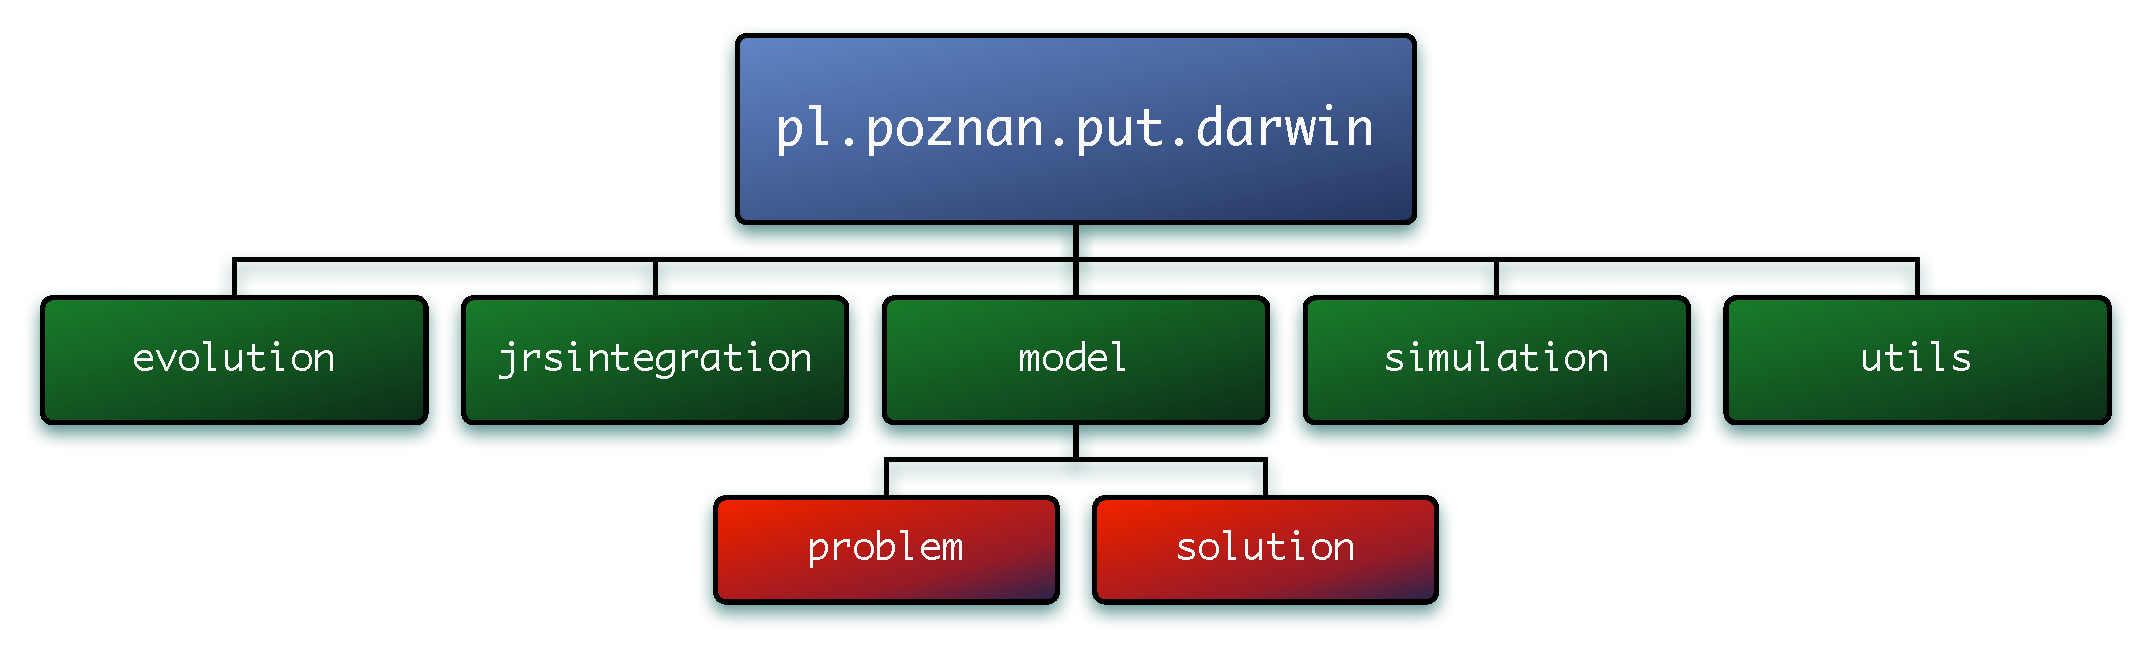
\includegraphics[scale=0.9]{img/packages}
  \caption{The package structure of DARWIN}
  \label{packages}
\end{figure}

The DARWIN code is divided into packages. Their structure is shown in
fig.~\ref{packages}. Their description follows. \texttt{pl.poznan.put.darwin}
is a~root package following Java naming conventions ([ref]). For readability
its name is omitted in the following description. Packages:
\begin{description}
  \item{\texttt{evolution}} --- a module containing classes responsible for
    the evolution of solutions. It contains a~controller driving the process,
    an engine of the evolutionary algorithm, evolutionary operators (mutation
    and cross-over) and a~parent selection strategy.

  \item{\texttt{jrsintegration}} --- an abstraction layer over the DRSA
    framework. This module contains classes responsible for integration with
    jRS and DomLem algorithm. They are able to convert DARWIN's solutions to
    a~format required by the jRS, invoke the DomLem algorithm and later ---
    during the interior loop --- check if a given solution matches any of the
    generated rules.

  \item{\texttt{model}} --- models a hierarchy of objects for an abstract MOO
    problem. Contains basic classes required to represent a~problem, its
    variables, goals and constraints, as well as classes representing
    a~solution and a scenario of uncertainty. A~problem parser --- for reading
    problem instances from files, a~solution evaluator --- computing a value
    of solution against given scenarios and a~configuration reader --- setting
    DARWIN's options on the basis of a file, are also components of the
    \texttt{model} package.
  \item{\texttt{simulation}} --- a package responsible for connecting all the
    other parts together. It initializes the process by asking \texttt{model}
    to read the problem and the configuration; takes care of the interaction
    with the DM, invokes \texttt{jrsintegration} to process the preferences
    and to obtain the rules and finally interacts with the evolution
    controller from the \texttt{evolution} package. It can also mock the
    decision maker and generate reports if needed for automated experiment
    framework.

  \item{\texttt{utils}} --- additional utility classes for the other modules.
\end{description}

In order to reduce the number of bugs and eliminate recurring of the fixed
bugs an extensive test suite accompanies each of the packages. In order to
streamline the building process the Scala Build Tool (SBT, see~[ref]) is used
to manage dependencies, to take care of running the test suite and to build
the application from its source code. The code contains javadoc ([ref]) on
most of the API methods and a lot of comments in places that could be
particularly hard or tricky to understand. Therefore it should be possible for
the other developer to use and extend the code delivered as a~part of the
thesis. A manual for the end-user is enclosed at the end of the paper.

A~lot of DARWIN parameters are mentioned throughout the paper. They are gathered
and described in table~\ref{t:params}. The parameters can be set in a
configuration file. The options are split into sections and listed in the
table. The syntax of the configuration file is described in the user manual
([inref]).

\begin{table}
  \centering
  \begin{tabular}{l l p{7cm} l}
    \hline
   Section &  Name & Description & Default value \\
    \hline
    \hline
    \multirow{15}{*}{Main} & 
    Solution count & The number of solutions in a population. & 30 \\
    & Scenario count & The number of scenarios on which the solutions will be evaluated.  & 30 \\
    & Generation count & The number of generations in the interior loop. & 30 \\
    & Gamma ($\gamma$) & The coefficient of elitism. The higher $\gamma$, the
      higher the probability of choosing a solution with a~higher rank as
      a~parent. & 2.0  \\
    & Delta ($\delta$) & The decay of rule weight (see [inref]). & 0.1  \\
    & Eta ($\eta$) & The initial mutation probability.  & 0.5    \\
    & Omega ($\omega$)& The decay rate of the mutation probability. & 0.1  \\
    & Outer count & The number of exterior loop iterations to be mocked. & 20 \\
    & Use average & Whether an average in quantiles should be used instead of
      the maximum value (see~[inref]). & false  \\
    & Mutation tries & The number of mutation tries. For some problems it may be
      very hard to mutate a solution to get the other feasible one. Try no more
      times than defined here.  & 20  \\
    & Use ``at most'' & Whether an ``at most'' rules should be considered
    along with ``at least'' (see~[inref]). & true \\
    & Percentiles & Which percentiles are meaningful to the decision maker. & 1.0, 25.0, 50.0  \\
    & Multi rules & Should the rules be generated multiple times (see~[inref]). & false \\
    & Multi rules count & How many iterations of rules generation should be performed. & 3 \\
    \hline
    DomLem & Confidence level & A level of confidence that the rules generated by the
    DomLem algorithm should at least have. & 1.0 \\
    \hline
    \multirow{3}{*}{MockedDM} & Base good count & The number of solutions to be marked
    as good by the mocked DM. & 3 \\
    & Good count delta & A parameter for simulating noise in DM's decisions. See~[inref]. & 2 \\
    & Noise level & A parameter for simulating noise in DM's decisions. See~[inref]. & 0 \\
    \hline
    \multirow{3}{*}{Evolution} & Regenerate every & During the interior loop
    the solution set is evaluated against a scenario set. This parameter
    specifies how often the scenario set should be changed --- in how many
    generations a regeneration of the set should occur. & 1000 \\
    & Regenerate percent & Part of the scenario set to regenerate. & 0.0 \\
    & Use supposed utility & If the evolutionary algorithm should use the
    supposed utility instead of a rule-based score. & false \\
  \hline
  \multirow{3}{*}{Reports} & Evolution report & If the set specifies where an
  evolutionary report should be written.  & \texttt{evrep.csv} \\
  & DM Report & If the set specifies where the DM's decision should be reported. & \texttt{dmrep.csv} \\
  &  Brief report & If a brief report should be written to standard
  output. Useful in supervising a batch run. & true \\
  \hline
  \end{tabular}
  \caption{The parameters of DARWIN}
  \label{t:params}
\end{table}


\section{Experiment framework}
One of the goals of the thesis was to evaluate the DARWIN's performance and
the importance of the parameters. To do this a set of tools was
developed. Firstly, DARWIN can be instructed to log details of an execution to
a file (see table~\ref{t:params}). These logs consist of two reports --- the
evolution report and the DM's decisions report. The former contains the
information about the population's shape and the latter about the decisions
made by the decision maker. The reports are in the comma separated values
format (CSV, [ref]).

The algorithm is interactive which means that constant human supervision is
required. However, one needs to repeat the experiments over and over
again. For this reason the decision maker has been mocked. It is possible to
pass a~utility function for a supposed decision maker and then, the algorithm
will make a~decision on its own on the supposed utility basis. This automates
a~single run of DARWIN, however an operator is still required to start the
program over and, if necessary, to change the execution parameters.

To bypass this limit and streamline the process, the experiment framework is
provided. One can define a base configuration along with a~test plan and then
a computer will proceed with an execution of the test plan. Scripts composing
the framework are written in Python --- a general, high-level programming
language and glued together using the Bash shell scripts
([ref]). A~description on how to use the framework is provided as a~part of
the user manual ([ref]).

A test plan execution will typically result in a~number of report files full
of the runs' details. It would be a tremendous task to analyze them by
hand. However, presenting this data in an aggregated form as a set of charts
can immensely simplify the analysis.

R is an environment for statistical computing ([ref]). The program along with
ggplot library ([ref]) has been used for the automatic chart generation. The R
scripts can import the CSV reports, aggregate and process the data and finally
generate a~chart. The whole experiment process is presented in
fig.~\ref{framework}.

First, a user prepares a~test plan and sends it to the framework. The
framework is repeatedly running DARWIN with a~mocked decision maker. Resulting
reports are then processed by the R~scripts. As a result charts are generated.

\begin{figure}
  \centering 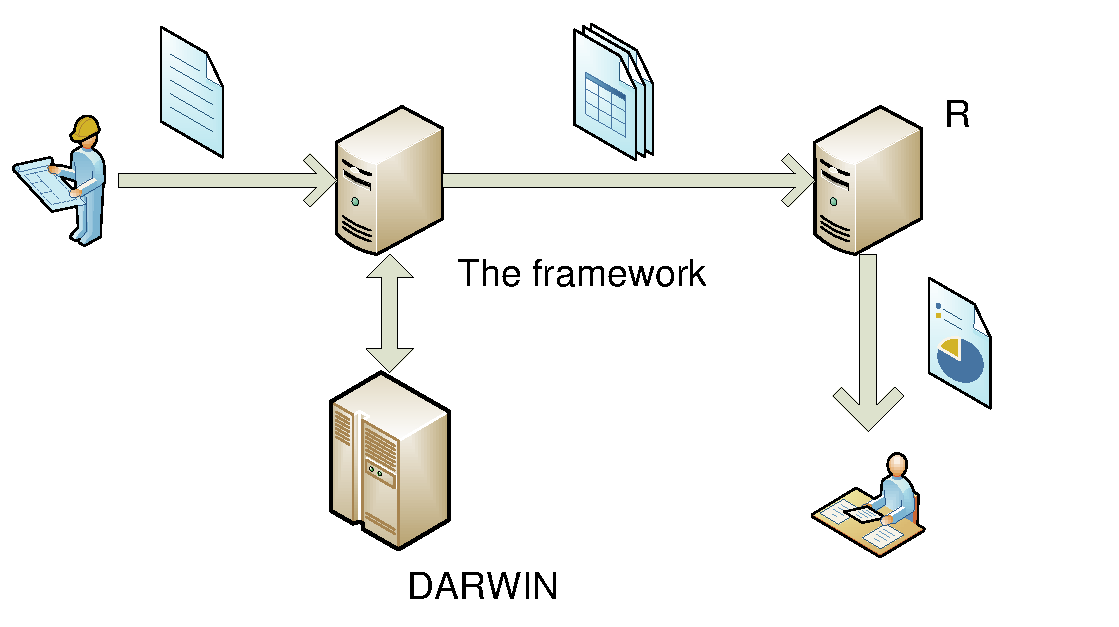
\includegraphics[width=\textwidth]{img/framework}
  \caption{The experiment process}
  \label{framework}
\end{figure}

It is possible to generate the following type of charts (they are shown in
fig.~\ref{chart_examples} and \ref{chart_examples2}).
\begin{itemize}
\item A change of the utility value during the exterior loop
  iterations. Example shown in fig.~\ref{ch_ex_a}. This is a basic chart for
  the analysis, because it shows a high-level overview of the run from the
  decision maker's perspective.
\item A change in a~population shape during the interior loop run. May show a
  convergence of a population to a specific region. Fig.~\ref{ch_ex_b}.
\item A change of the utility value along with the primary score during the
  interior loop --- a run of the evolutionary algorithm. Fig.~\ref{ch_ex_c}.
\item Shows the change in a~population of an evolutionary algorithm from the
  utility and the primary score perspective. Fig.~\ref{ch_ex_b}.
\item A comparison chart --- to present the utility value change of multiple
  tests (possible with different parameters) side-by-side. Each test
  consists of one or more runs. Fig.~\ref{ch_ex2_a}.
\item A comparison chart --- to compare the results of several tests. Each
  test consists of several runs. The results are charted on a box plot, so the
  analyst can easily compare a median, the first and the third quartile and
  outliers of each test. Fig.~\ref{ch_ex2_b}.
\item A chart showing decision maker's selections. Whole presented population
  is shown and selected individuals are marked. Fig.~\ref{ch_ex2_c}.
\end{itemize}

\begin{figure}
  \centering
  \makebox[\textwidth]{
    \subfloat[Exterior loop iterations $\rightarrow$ the utility value]{
      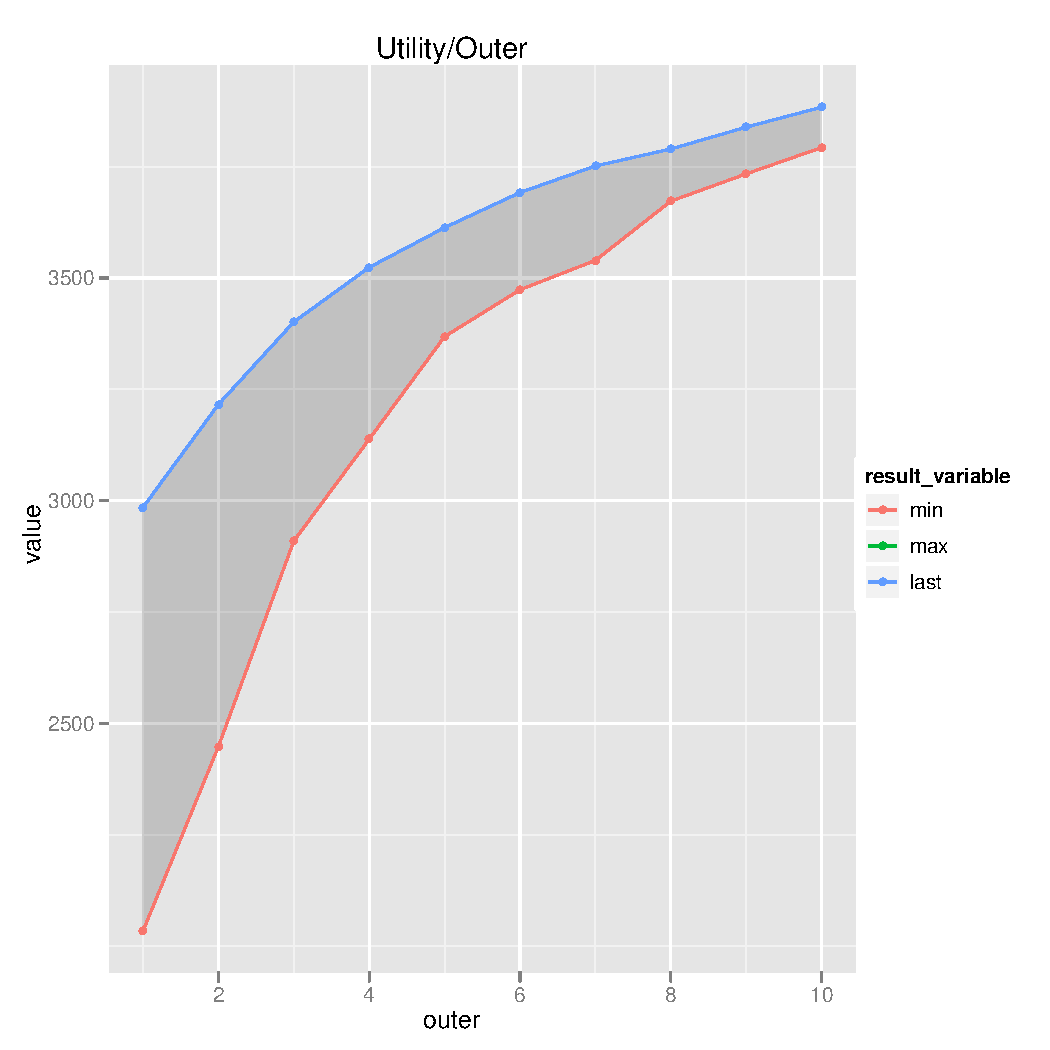
\includegraphics[width=0.65\textwidth]{charts/utilouter}
      \label{ch_ex_a}
    }
    \subfloat[The population shape change]{
      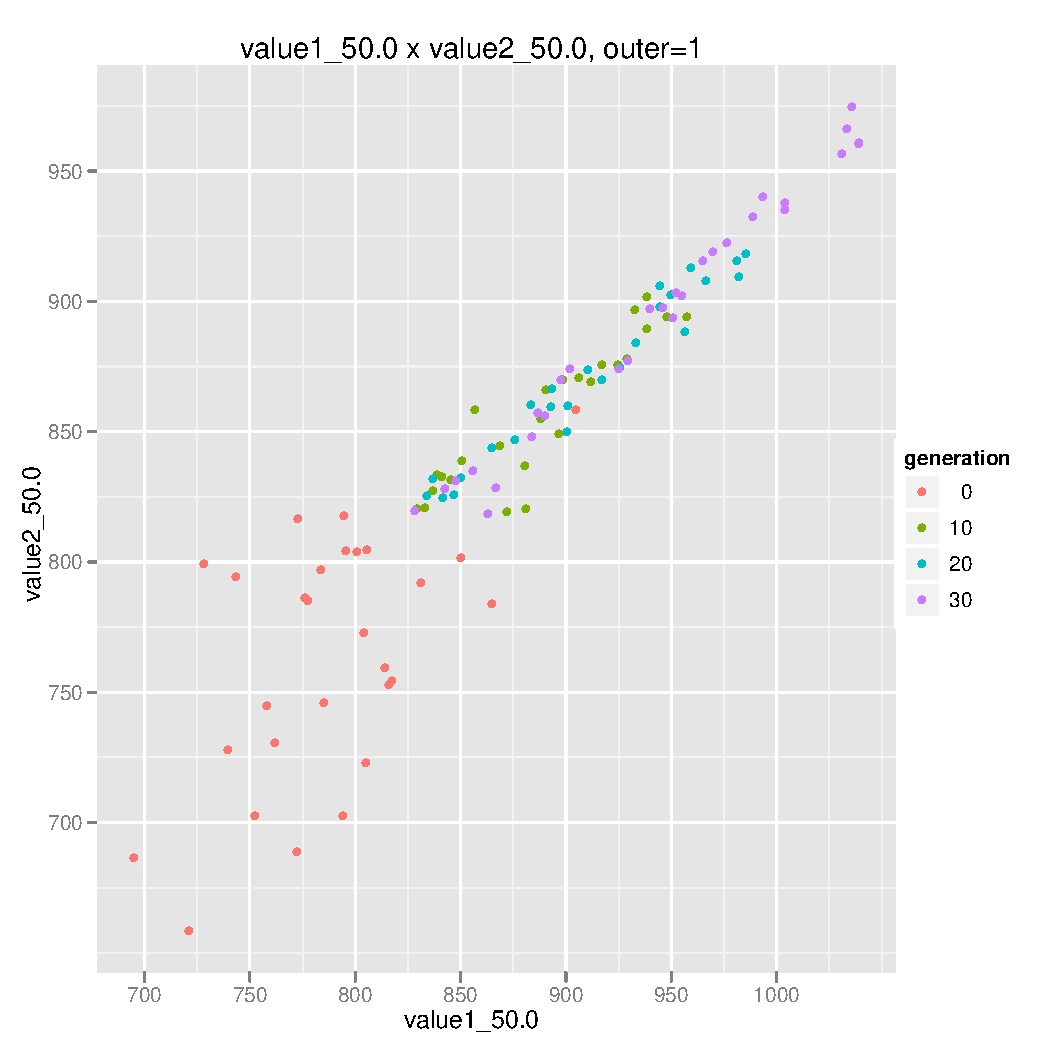
\includegraphics[width=0.65\textwidth]{charts/valweight_01}
      \label{ch_ex_b}
    }
  }
  \makebox[\textwidth]{
    \subfloat[Interior loop generations $\rightarrow$ the utility value, the primary score]{
      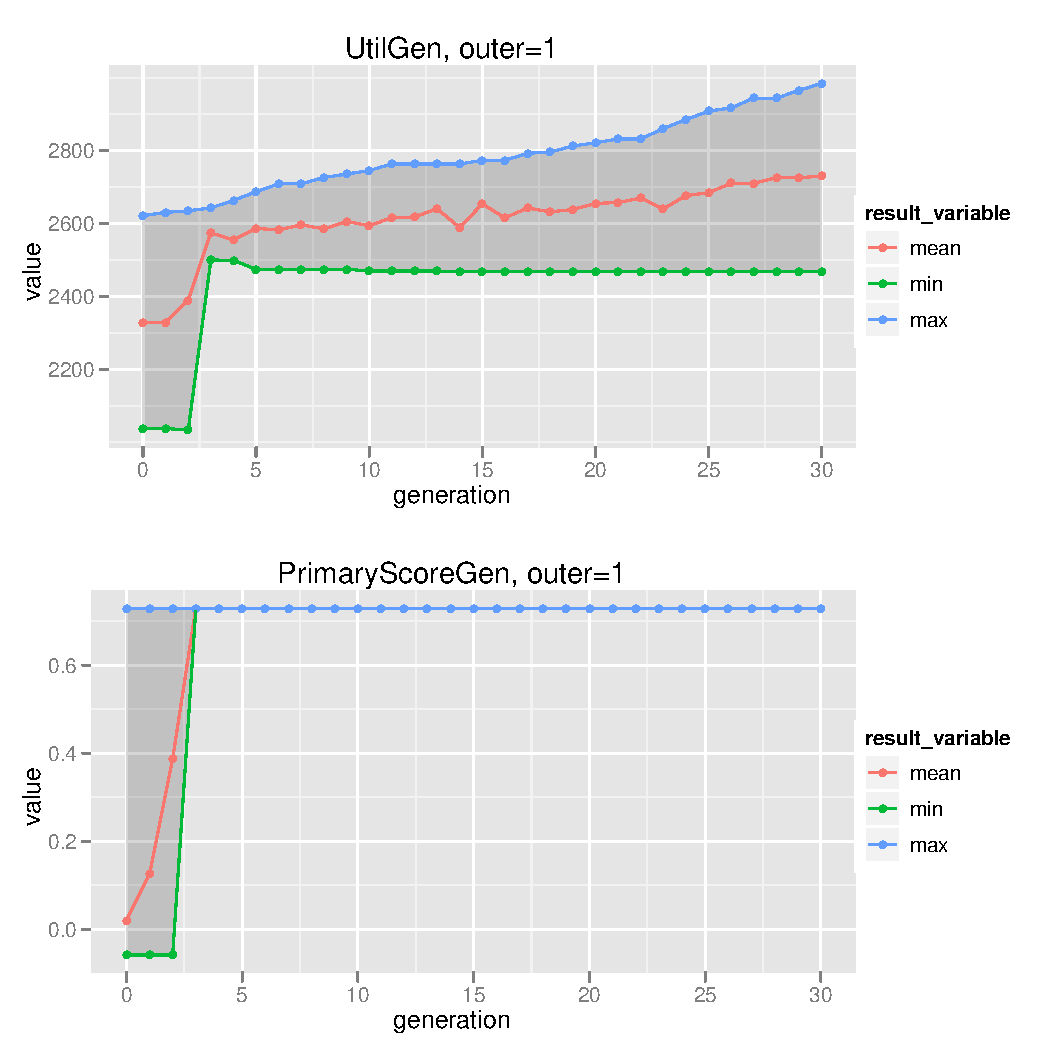
\includegraphics[width=0.65\textwidth]{charts/utilgen_01}
      \label{ch_ex_c}
    }
    \subfloat[The change of the utility and the primary score in a population]{
      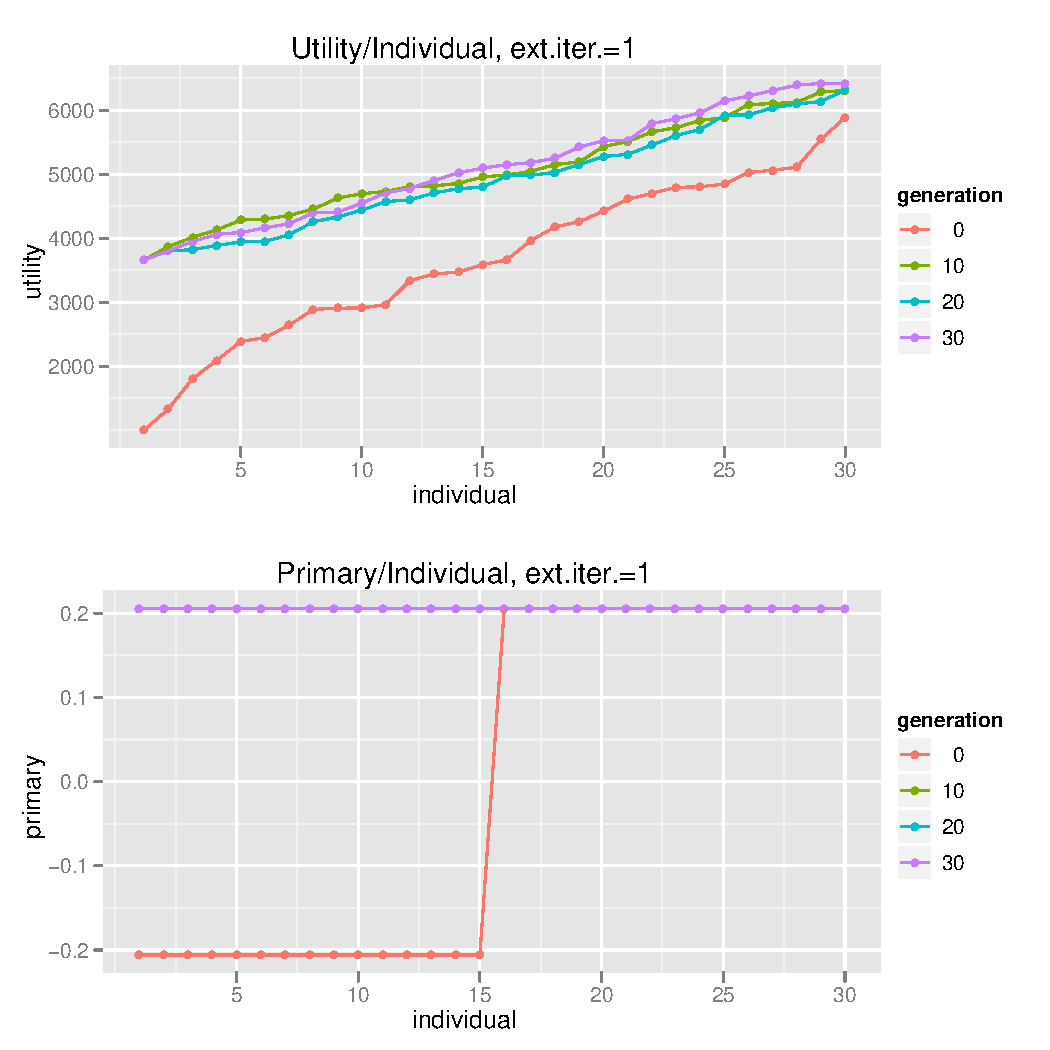
\includegraphics[width=0.65\textwidth]{charts/utilind_01}
      \label{ch_ex_d}
    }
  }
  \caption{Type of charts available in the experiment framework}
  \label{chart_examples}
\end{figure}

\begin{figure}
  \centering
  \makebox[\textwidth]{
    \subfloat[The comparison of test runs]{
      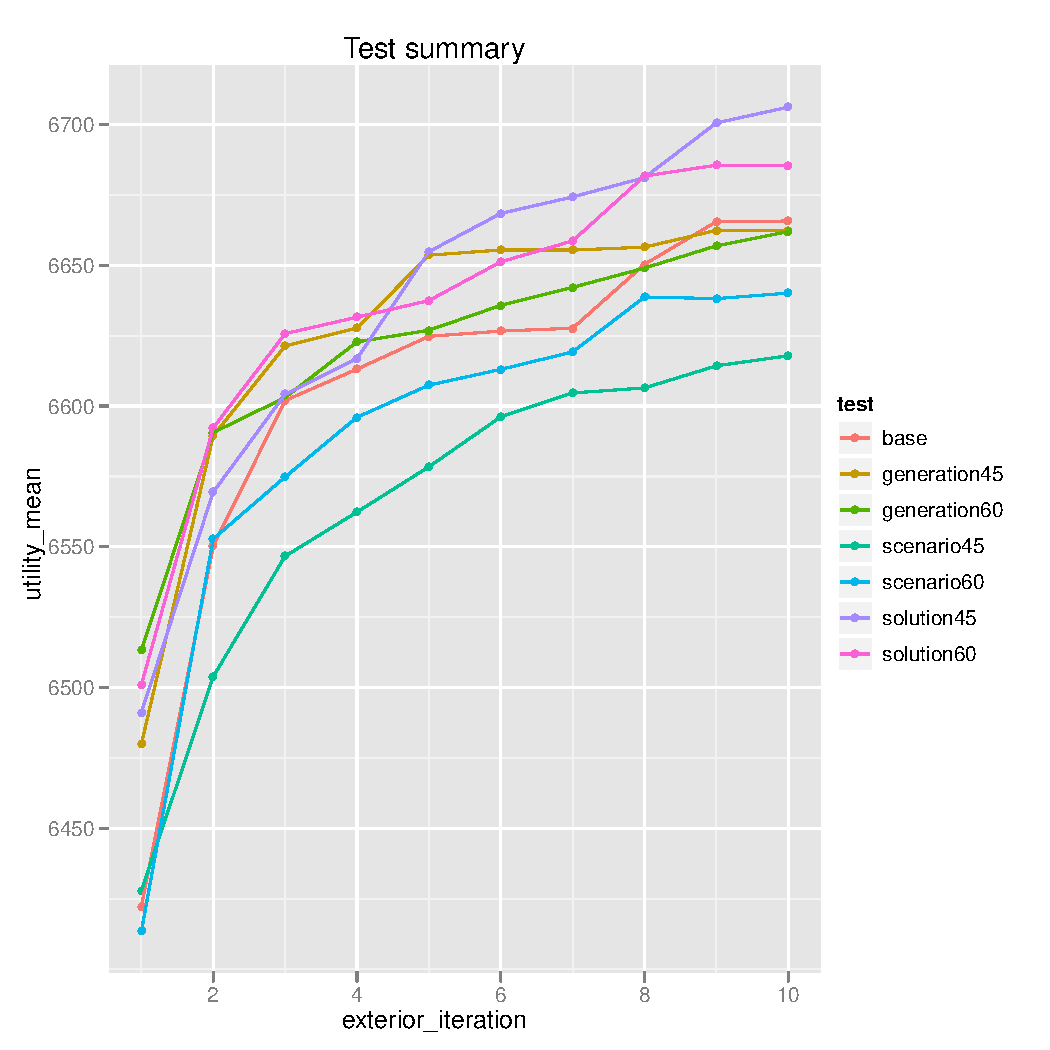
\includegraphics[width=0.65\textwidth]{charts/summary1}
      \label{ch_ex2_a}
    }
    \subfloat[The comparison of test runs]{
      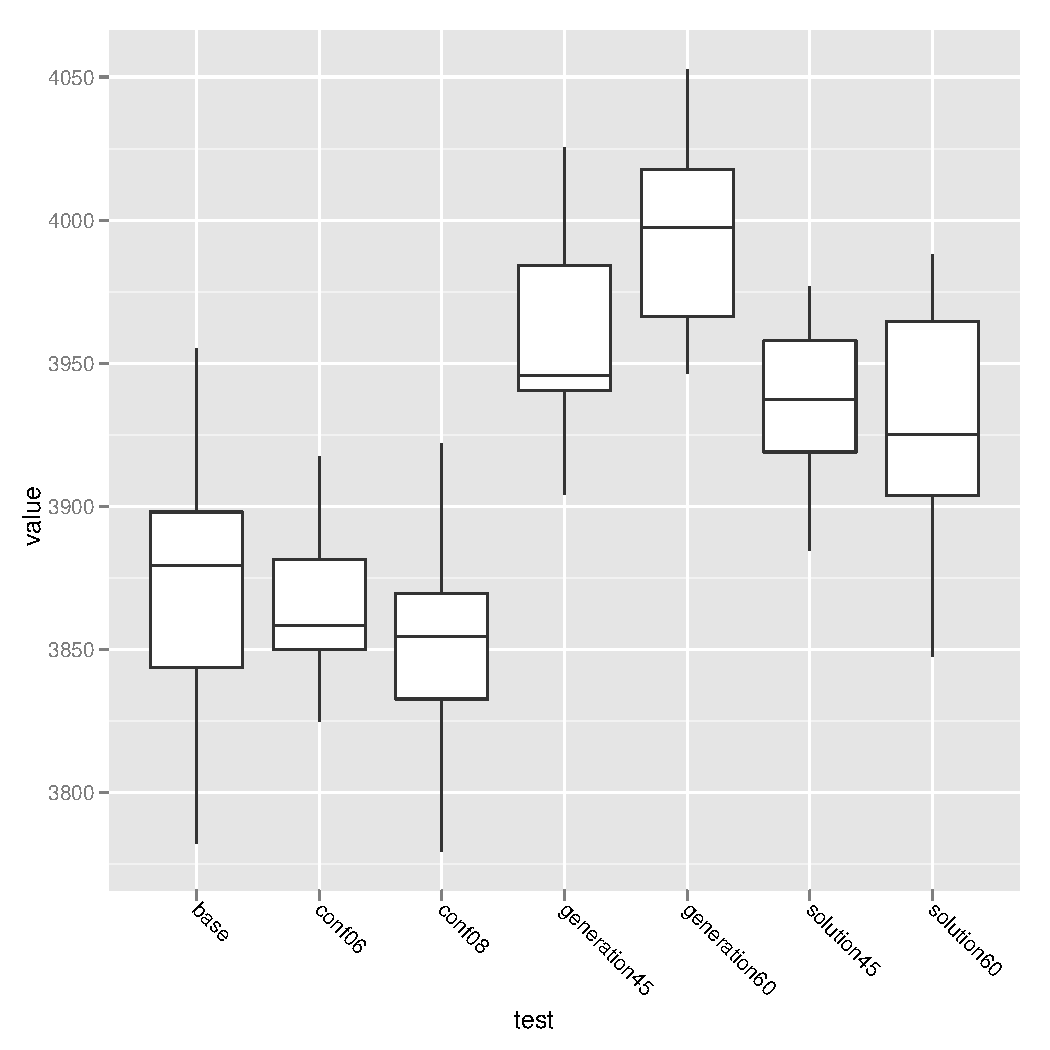
\includegraphics[width=0.65\textwidth]{charts/summary2}
      \label{ch_ex2_b}
    }
  }
  \makebox[\textwidth]{
    \subfloat[The decision maker choices]{
      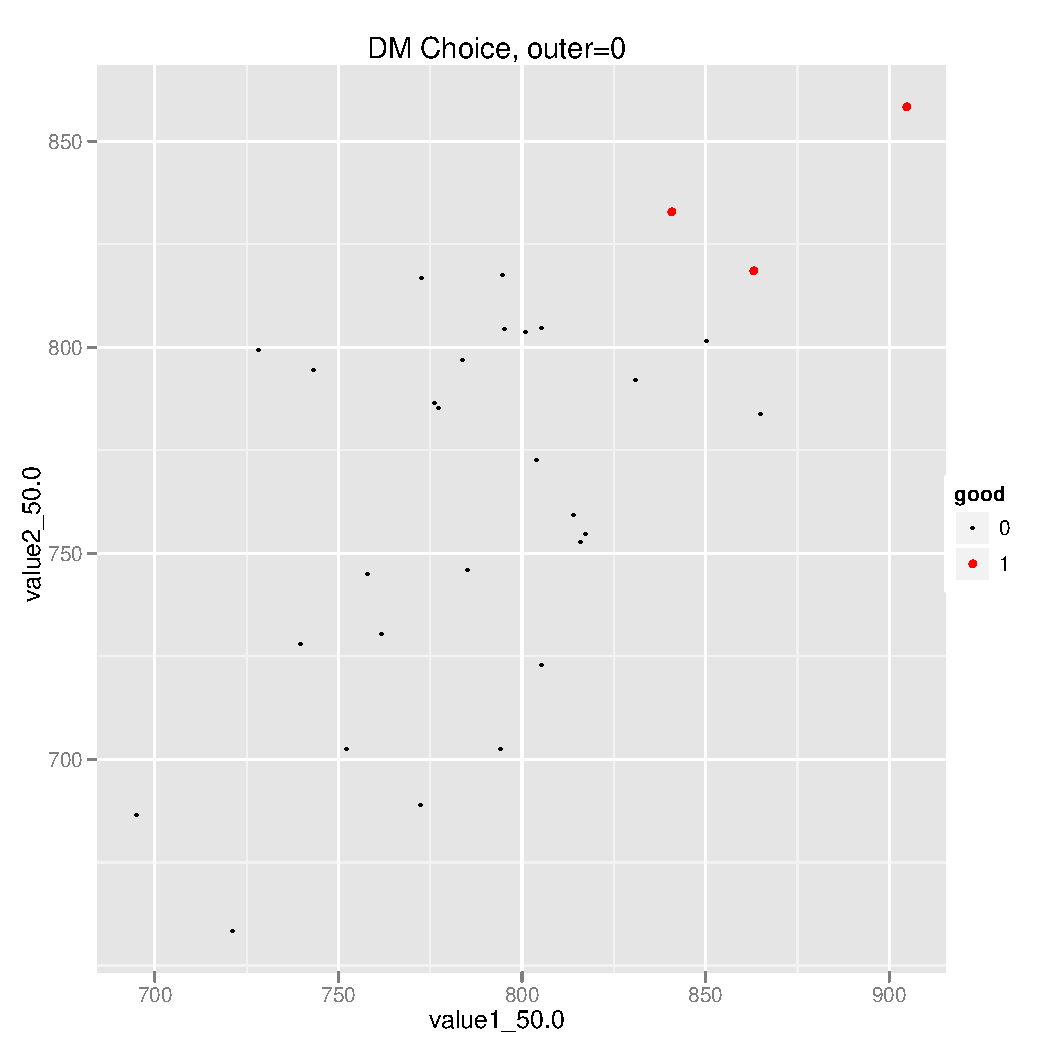
\includegraphics[width=0.65\textwidth]{charts/dm_choices_01}
      \label{ch_ex2_c}
    }
  }
  \caption{Type of charts available in the experiment framework}
  \label{chart_examples2}
\end{figure}

The framework is just a utility, but still an important one to evaluate the
performance of the method. The implementation presented in this chapter was
a~basis for the DARWIN method's evaluation. The results are given in the next
chapter.
